\chapter{Interface Utilisateur}\label{cha:interface}
Ce chapitre présente les concepts fondamentaux de l'interface utilisateur de XCSoar. Les chapitres suivants fourniront des détails quand cela sera nécessaire.

\begin{center}
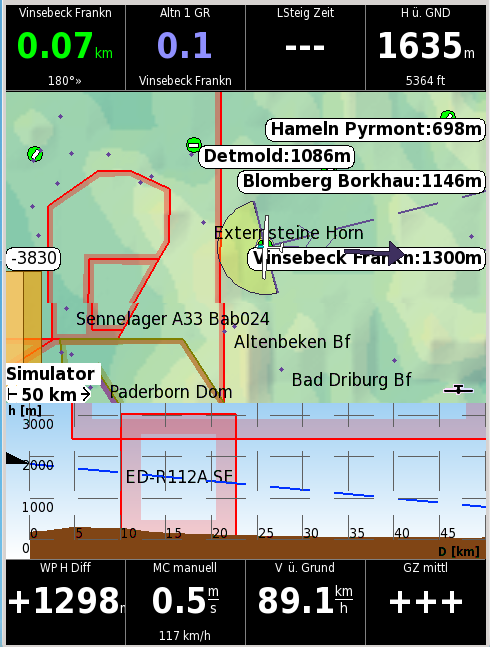
\includegraphics[angle=0,width=\linewidth,keepaspectratio='true']{figures/plain.png}
\end{center}

L'affichage est composé de plusieurs éléments :
\begin{description}
\item[La carte] La plus grande partie de l'écran est dédiée à l'affichage de la carte mobile. Différents symboles du calculateur de vol sont superposés sur la carte. Des icônes et des textes peuvent apparaitre en bas de l'écran pour indiquer l'état de connexion des appareils reliés au calculateur, le mode utilisé, ....
\item[InfoBoxes] Ces "boites d'information" sont présentées comme sur une grille ou damier : en haut et en bas de l'écran (en mode portrait), de chaque côtés de l'écran (en mode paysage). Ces InfoBoxes affichent les données calculées par XCSoar, celles du GPS et celles des instruments connectés au calculateur.
\item[Instruments]  Affichage des des instruments. Ils sont tous optionnels et certains n'ont de véritable utilité que connecté à un instrument externe supporté.
\item[Boutons et menus] Les boutons/touches du matériel sur lequel est installé XCSoar permettent de faire apparaitre des menus sur l'écran t de naviguer dans ces menus à l'aide des touches adjacentes. Si l'appareil a un écran tactile, la navigation se fait en touchant les boutons sur l'écran. Ces boutons ont un fond gris clair et un texte noir.
\item[Messages d'état] Le texte des messages d'état sont affichés par dessus la carte. Ce texte est utiliser pour informer le pilote de certains évènements.
\item[Panels de dialogue] Ce sont de grandes boites de dialogue, contenant en général des données détaillées, des graphiques et des boutons....
\item[Menu principal] Le menu principal apparait en appuyant 2 fois sur la carte ou sur les InfoBoxes et aussi par geste sur la carte \gesture{Haut - Bas}. Si les boutons ne sont pas utilisés après un certain temps, ils disparaissent afin de rendre la carte visible entièrement.
\end{description}

Plusieurs façons d'inter-agir avec XCSoar :
\begin{itemize}
\item En touchant certains éléments de la carte.
\item En touchant les InfoBoxes et les boutons des menus.
\item Par 'Gestes' : en traçant des formes avec le doigt, par exemple un trait de gauche à droite.(voir section  \ref{sec:gestures} ci-dessous).
\item 'En tirant' sur l'écran ( toucher + déplacer le doigt + relâcher).
\item En appuyant sur des boutons, de l'appareil, gérés par l'application.
\item En appuyant sur les touches déplaçant le curseur de l'appareil.
\item En appuyant sur les touches/boutons d'un instrument connecté à XCSoar.
\end{itemize}
En fonction du matériel sur lequel XCSoar est installé, toutes ces méthodes ne sont pas obligatoirement possibles et certains boutons peuvent avoir différentes fonctions.

Pour la version PC de XCSoar, cliquer sur un élément de l'interface utilisateur revient à le toucher sur un écran tactile.

Altair n'ayant pas d'écran tactile, toutes les inter-actions se font à l'aide des boutons physiques, des switches ou boutons de commande des matériels connectés.

\section{Menu Principal}

Le menu principal est un ensemble de boutons affichés à l'écran. Ils s'utilisent par toucher (pression sur l'écran) ou par pression sur des touches physiques, suivant le matériel. Faire apparaitre/disparaitre le menu principal et naviguer dans les sous menus représente la base de l'utilisation de XCSoar.

\subsection*{Les bases de l'interface utilisateur}
Le menu est organisé en quatre groupe de fonctions, en général hiérarchisées.La disposition des menus est liée au matériel sur lequel est installé XCSoar. Cette disposition des menus peut aussi être personnalisée par l'utilisateur.

XCSoar gère aussi des signaux d'entrée en provenance de claviers, manettes de jeux, joysticks, ... Une grande variété de fonctions peuvent leur être assignées.
\sketch{figures/buttonmenu.png}
Pour Altair, il y a quatre boutons principaux qui sont activés en appuyant sur les touches verticales de côté gauche. Quand un menu est activé, une bande de boutons apparait le long du bord bas de l'écran. Un nouvel appui sur le bouton permet de se déplacer d'une page (constituée d'éléments) à la suivante. L'appui sur le bouton horizontal correspondant active l'élément choisi. A la dernière page, l'appui sur le bouton de menu enlève tous les boutons affichés.

Sur la version PC, ces menus sont activé par les touches 1, 2, 3 et 4. 3. Les touches 6, 7, 8, 9 et 0 corresponde à la bande de boutons horizontale en bas de l'écran.

Sur la version PDA, les menus sont activés à l'aide des touches qui sont à côté du bouton rocker/joystick.

Si il n'y a pas d'interaction avec le calculateur pendant un certain temps, les menus disparaissent automatiquement. Cette durée est paramétrable. La touche Echap./ESC sur PC ou PWR/ESC sur Altair peuvent aussi être utilisées pour fermer les menus. 

Les boutons peuvent apparaitre grisés si la fonction correspondante n'est pas disponible. Par exemple, la liste des points de virage apparaitra grisée si aucun point n'a été chargé.

Plusieurs boutons comportent des textes dynamiques. Ceci dans le but de rendre plus compréhensible ce qui se passera quand on appuiera dessus. Par convention, le texte du bouton indique l'action effectuée quand on appuie sur le bouton. Par exemple, le bouton \bmenu{MC Auto} montre que si on appuie dessus, alors le paramètre "MacCready Auto" sera sur ON. Si on appuie dessus, le texte du bouton devient alors \bmenu{MC Manuel}. Dans la liste des menus qui suit, les labels génériques sont utilisés.

\subsection*{Quatre menus principaux}
Voici la disposition des menus principaux sur toutes les plateformes sur lesquelles XCSoar peut-être installé. Les chapitres suivants donneront les détails de leurs sous menus.

Ces menus principaux sont activés sur Altair par les boutons verticaux, de haut en bas :
\begin{jspecs}
\item[\bmenu{Nav.}] Regroupe les contrôles de navigation et les circuits.
\item[\bmenu{Affich.}] Regroupe les contrôles de l'affichage.
\item[\bmenu{Config.}] Configuration/paramétrage de XCSoar, des appareils connectés et des paramètres de vol.
\item[\bmenu{Info.}] Ouverture de diverses boites de dialogue d'information. 
\end{jspecs}

Pour la version PC, les touches 1, 2, 3 et 4 ouvrent les menus correspondants. La liste des sous menus qui suit comporte des liens pour presque chaque élément. Cliquez dessus pour arriver directement sur les informations détaillées correspondantes.

\section{Menu item overview}

\subsection*{Navigation menu}
\noindent\makebox[\textwidth]{%
\begin{tabularx}{1.8\textwidth}{l|ccccc}

Nav 1
 & \ref{cha:tasks}\bmenus{Task}
 & {\bmenut{Previous}{Turnpoint}}
 & {\bmenut{Next}{Turnpoint}}
 & \ref{sec:waypoint-selector-dialog}\bmenut{Waypoint}{List}
 & \ref{sec:alternates}\bmenus{Alternates} \\ \\
Nav 2
 & \ref{sec:taskabort}\bmenut{Task}{Abort}
 & \ref{sec:markers}\bmenut{Mark}{Drop}
 & {}
 & \bmenus{Target}
 & \ref{sec:waypointdetails}\bmenut{Waypoint}{Details}

\end{tabularx}}

You should not start using XCSoar without knowing about the `Alternates' feature. 
Any `Task' related item in the navigation menu are used for planned cross 
country flight and certainly the second step.

\subsection*{Display menu}
\noindent\makebox[\textwidth]{%
\begin{tabularx}{1.9\textwidth}{l|ccccc}

Display 1
 & \ref{sec:zooming}\bmenut{Zoom}{In}
 & \bmenut{Zoom}{Out}
 & \bmenut{Zoom}{Auto}
 & \bmenus{Info Cruise}
 & \ref{sec:panning}\bmenut{Pan}{On} \\ \\
Display 2
 & \ref{sec:maplabels}\bmenut{Labels}{All/...}
 & \ref{sec:trail}\bmenut{Trail}{Full/...}
 & \ref{sec:terrain_topo}\bmenut{Terrain}{On/Off}
 & \ref{sec:terrain_topo}\bmenut{Topo.}{On/Off}
 & \ref{sec:terrain_topo}\bmenut{Airspace}{On/Off}
 

\end{tabularx}}

Most of the display menu items are available on gestures, or special key 
short-cuts of your device. Once you are familiar with XCSoar you probably 
will use those menu items less frequently.

\subsection*{Configuration menu}
\noindent\makebox[\textwidth]{%
\begin{tabularx}{1.9\textwidth}{l|ccccc}

Config 1 & \bmenut{MacCready}{$+$} & \ref{sec:stf}\bmenut{MacCready}{$-$}
 & \ref{sec:auto-maccready}\bmenut{MacCready}{Auto}
 & \ref{sec:flight-setup}\bmenut{Flight}{Setup}
 & \ref{sec:wind-setup}\bmenut{Setup}{Wind} \\ \\
Config 2 & \bmenus{Vega}
 & \ref{cha:configuration}\bmenut{Setup}{System}
 & \ref{sec:airspace-filter}\bmenut{Settings}{Airspace}
 & \ref{sec:logger}\bmenut{Logger}{Start}
 & \ref{sec:logger-replay}\bmenus{Replay} \\ \\
Config 3 & \ref{sec:raw-logger}\bmenus{Raw Logger}
 & \ref{conf:comdevices}\bmenus{Devices}
 & \bmenut{Setup}{Plane}
 & \bmenut{File}{Manager}

\end{tabularx}}

The configuration menu is typically part of the ground interaction with 
XCSoar. You are not expected to spend much time in-flight with tweaking 
the configuration, except you manually adjust wind or MacCready settings. 
The `Vega' item gives control over the  Vega intelligent variometer. This 
comprises a sub-menu.


\subsection*{Information menu}
\noindent\makebox[\textwidth]{%
\begin{tabularx}{1.8\textwidth}{l|ccccc}

Info 1 & \ref{sec:flarm-traffic}\bmenut{FLARM}{Radar}
 & \bmenut{METAR}{TAF} & \bmenut{What's}{here?}
 & \ref{sec:checklist}\bmenut{Check}{list}
 & \ref{sec:analysis-climb}\bmenus{Analysis} \\ \\
Info 2 & \ref{sec:flight-status}\bmenus{Status}
 & \ref{sec:weather-forecast}\bmenus{Weather}
 & \ref{sec:team-flying}\bmenut{Team}{Code}
 & \bmenut{FLARM}{Details}
 & \ref{sec:team-flying}\bmenut{Thermal}{Assistant} \\ \\
Info 3 & \ref{sec:credits}\bmenus{Credits}
 & \bmenut{Message}{Repeat}

\end{tabularx}}

The information menu is always a good address, when not only a clue on 
how to set MacCready is requested, but rather more elaborate help on a 
larger scope tactical decision on your flight is requested.


\subsection*{The Vega variometer sub-menu of the configuration menu}

\noindent\makebox[\textwidth]{%
\begin{tabularx}{1.8\textwidth}{l|ccccc}

Vega 1 & \bmenut{Airframe}{Switches} & \bmenut{Setup}{Audio}
 & \bmenut{Manual}{Demo} & \bmenut{Setup}{Stall} & \bmenus{Accel} \\ \\
Vega 2 & \bmenut{ASI}{Zero} & \bmenut{Accel}{Zero}
 & \bmenus{Store} & \bmenut{Cruise}{Demo} & \bmenut{Climb}{Demo}

\end{tabularx}}

The functions in this sub-menu require the Vega intelligent variometer. 
The menu can only be accessed if `Vega' is selected as the connected device.

\subsection*{The pan mode sub-menu of the Display menu}

\noindent\makebox[\textwidth]{%
\begin{tabularx}{1.6\textwidth}{l|ccccc}
Pan & \bmenut{Pan}{Off} & \ref{sec:panning}\bmenut{Zoom}{in} & \bmenut{Zoom}{out}
 & \bmenut{What's}{here?}
\end{tabularx}}

This sub-menu unfortunately overlays the full-screen map view of the pan mode.
 It's functions are quite evident, although the menu could be replaced by multi-touch
 technology or knobs (like on Altair). Besides the essential `exit pan mode'
 function the `What's here?' button offers brilliant access to the variety of
 information of the map.

\section{Default menu buttons}

When no menu is active, (so-called default mode), the horizontal row
of buttons in Altair perform the following functions (from left to right):

\begin{center}
\begin{tabular}{c c c c c c}
 PC: & 6 & 7 & 8 & 9 & 0 \\
 Altair: & F5 & F6 & F7 & F8 & F9 \\
& \bmenut{Flight}{Setup} & \bmenut{Task}{Manager} & {} &
\bmenus{Target} & \bmenut{Drop}{Mark} \\
\end{tabular}	
\end{center}

Pressing ESC on Altair displays labels for these default menu buttons.

For all other versions in the default mode, the cursor keys perform
the following functions:
\begin{jspecs}
\item[Up key] Zoom in
\item[Down key] Zoom out
\item[Left key] Drop marker
\item[Right key] Toggle through normal/aux. InfoBoxes and full-screen
\item[Enter] Clear status message or suppress FLARM gauge if open and no warning
active
\end{jspecs}

For the Altair version in the default mode, the rotary knob performs
the following functions:
\begin{jspecs}
\item[Outer knob counter-clockwise] Zoom in
\item[Outer knob clockwise] Zoom out
\item[Inner knob counter-clockwise] (No function assigned)
\item[Outer knob clockwise] (No function assigned)
\item[Knob button press] Clear status message or acknowledge airspace warning
\end{jspecs}

In dialogue forms, the rotary knob in Altair performs the role of the cursor and
enter keys:
\begin{jspecs}
\item[Outer knob counter-clockwise] Up cursor
\item[Outer knob clockwise] Down cursor
\item[Inner knob counter-clockwise] Left cursor
\item[Inner knob clockwise] Right cursor
\item[Knob button press] Enter key
\end{jspecs}

For Altair, the buttons along the edge of the display can be used as
alternate ways of navigating in dialogues.  The F4 key (directly above
the rotary knob) can be used as an alternate ENTER key (instead of
pressing the rotary knob) in dialogues.  The F6 and F7 keys (directly to
the right of the rotary knob) can be used to select the next or
previous page in multi-page dialogues.

\subsection*{Dynamic menu labels}
Certain menu items have dynamic labels to make it clearer what happens when the
menu item is selected.  Furthermore, items that are not available are greyed
out to indicate that selecting the menu item will not do anything.

The convention used for dynamic menu labels is for the labels to display the
action that will be performed once the menu item is selected. For example 
``Lights On'' will turn the lights on, and the menu will be updated to display
``Lights Off'', which would then if pressed turn the lights off. This
convention is used throughout XCSoar.

A selection of key dynamic menu items is presented below:
\begin{description}
\item[\bmenu{Next Turnpoint}]  
  Greyed out if the task is cleared, or if the active turnpoint is the
  finish. If the currently active turnpoint is the turnpoint prior to the 
  finish, this displays  ``Waypoint finish''.
\item[\bmenu{Previous Turnpoint}]  
  Greyed out if the task is cleared, or if the active turnpoint is the
  start and there are no multiple start points.  If there are multiple
  start points and the active turnpoint is the start, then this
  displays ``Cycle start'' to allow selection between the various
  start points.  If the active turnpoint is the first turnpoint after 
  the start, this displays ``Waypoint Start''.
\item[\bmenu{Labels All}]  
  This will turn on all labels available on the map. There are more options to 
  only show a reduced set of labels like ``Labels Task'', thus not cluttering the 
  screen too much.
\item[\bmenu{Target}]  
  Greyed out if the task is cleared or in task abort.
\end{description}


\section{InfoBoxes and screen pages}

The information displayed in the InfoBox fields can be selected from a
wide variety of options (listed in Chapter~\ref{cha:infobox}). These
fields can also be used to change for example the MacCready setting.

The specific number and layout of the InfoBox grid depends on the
screen orientation and the device's display size.  

For a 320x240 display
Pocket PC in portrait mode, there are four InfoBoxes above and four
InfoBoxes below the map display.  
\sketch{figures/infoboxes.png}

A typical landscape layout has 9 InfoBoxes and the variometer gauge 
to the right of the map display. 
 
For larger displays are up to 24 InfoBoxes on one screen page possible.


\subsection*{Pages with different InfoBox sets}

XCSoar allows the pilot to define various sets of InfoBoxes that are 
appropriate to various stages of flight (e.g. when circling in a thermal, 
flying between thermals, on final glide, etc.). XCSoar can be configured 
to automatically switch from one screen page to another based on the mode 
of flight, or you can manually roll through the various pages, including 
one with a full-screen map and no InfoBoxes at all. Thus a screen page 
consists of a InfoBox set and specific map appearance, that includes 
map orientation and scale.

\gesture{Right or Left} 
To toggle through the various InfoBox pages, using the left/right cursor 
keys (Altair), or by gestures (touch-screen).


\subsection*{Modifying InfoBox content}

(This section applies only when a touch-screen or mouse is present.)

Some InfoBox values can be changed by the user by selecting (i.e. long-pressing) the
InfoBox with the touch-screen or mouse.  This brings up a small tabular dialogue:

\begin{description}
\item[\bmenu{Edit}]  
  Allows the pilot to adjust the InfoBox setting (e.g. raise or lower the 
  MacCready setting)

\item[\bmenu{Setup}]
  Allows you to change the behaviour of the setting related to the InfoBox 
  (for example, changing from auto to manual MacCready mode); or 
  to change the InfoBox itself by pressing `{\it Switch InfoBox}', then 
  choosing from a list of all available InfoBoxes.

\end{description}

Examples of InfoBoxes that can
be adjusted include MacCready setting, wind speed, and height (QNH).


\subsection*{Changing InfoBox sets}

An entire set of InfoBox can be composed by the `{\it Setup System}' configuration 
dialogues on the `{\it Look / InfoBox Modes}' and `{\it Look / InfoBox Pages}' 
\ref{sec:infobox_sets} setup page. 
The dialogues give a wide variety to setup the look and feel of the XCSoar pages.  


\section{Status messages}

Status messages appear over the map area to present text for a short period of
time.  The message disappears after the time period has elapsed, and different
types of message have different periods. Additionally, status messages can be
made to disappear by acknowledging the message.  Acknowledgement is achieved by
either pressing the enter key (rotary knob on Altair), touching the status
message (on touch-screen devices) or clicking the screen (mouse enabled devices).

Additional user buttons may be assigned to a status message repeat function,
which brings up the last message again.
\sketch{figures/status-message.png}

Typical status messages include:
\begin{itemize}
\item Airspace queries
\item Airspace warnings
\item User interface events (e.g.\ changing display modes)
\item Glide computer events (e.g.\ take-off, turning waypoints)
\end{itemize}

Note that status messages do not appear while a dialogue is on screen, the
messages are buffered and displayed as soon as the dialogue is exited.


\section{Dialogue windows}\label{sec:dialog-windows}

XCSoar contains several dialogue windows that can be activated to bring up
additional information and are also used for more complex interactions with the
user, such as editing tasks and configuring settings.

Some dialogues simply display information, and require no user input. Other
dialogues contain data fields that can be modified or buttons that can be pressed.  

A cursor appears over the active button or data field. Pressing the up/down
arrow keys (or rotating the outer knob on Altair), the cursor will cycle
through the next or previous items. For list items and scrollable text, the
up/down arrow key moves the cursor up or down the list or text, and the
left/right arrow keys move the cursor up or down by one page in long lists.

For PDAs and PC versions, list items can be selected by touching the item (or
left-clicking with the mouse). Once a list item is selected, another touch
(left click) is equivalent to pressing the enter key.

Pressing the right/left arrow keys (or rotating the inner knob on Altair), the
data field value under the cursor can be modified. Pressing the enter key (or
pressing the rotary knob on Altair) activates the button or makes a selection
from a list.

Dialogues are typically started from the button menu.  

Many of the dialogue windows have multiple pages of information and are controlled
in a consistent fashion. Press the \button{$<$} or \button{$>$} buttons to
select the next or previous page of the dialogue and the \button{Close} button to
make the dialogue disappear.

The escape key on a PC or the PWR/ESC button on Altair, can also be used to
close dialogues.

The user must close the dialogue to return to the map view. When a dialogue
has been opened, the main button menu is disabled until the dialogue is closed.

In some dialogues, items that are not relevant or valid (such as AAT details when
flying a non-AAT task) are not displayed.

A summary of the major dialogues is presented below.
\begin{description}
\item[Flight setup] Used to modify the polar of the glider both before and
during flight, as well as to set the QNH pressure
\item[Wind] Used to modify or adjust the estimated wind magnitude and direction
\item[Waypoint details] Describes a waypoint in detail and has navigation
functions such as `GoTo' and `Insert in Task'
\item[Waypoint list] Used to select a waypoint from the waypoint database
\item[Task manager] Used to create, modify and view cross country tasks
\item[Analysis] Shows several pages of analysis and statistics about the flight
\item[Status] The status dialogues give summaries of the situation of the 
aircraft, system, task, start and times
\item[Configuration] Allows XCSoar and certain connected devices to be
configured
\item[Airspace filter] Controls enabling and disabling the display and warnings
of each airspace class
\item[Team code] Allows transfer of coordinates between FLARM team mates via a 
  code
\item[Devices]  Selection of various external devices (e.g. smart variometers, 
  FLARM, etc.).
\item[Setup Plane]  Easy reconfiguration of the plane-dependant settings (e.g. 
  polar, competition ID, etc.) by choosing from a list of previously-created 
  plane profiles.
\end{description}

These dialogues are described in later chapters. with the exception of the
check-list, status and text entry dialogues, which are described below.


\subsection*{Check-list (dialogue example)}\label{sec:checklist}

The checklist dialogue can display several pages of user-defined free text.
Typically this is used for check-lists. It can be accessed via the menu.
\begin{quote}
\bmenus{Info 1}\blink\bmenut{Check}{List}
\end{quote}

These check-lists may include: daily inspection, preflight, out-landing,
\sketch{figures/checklist.png}
pre-landing, radio procedures, and aircraft rigging and de-rigging
instructions.  Since the check-lists may be long, the up/down keys (or rotary
knob on Altair) may be used to scroll through the text. Clicking the
\button{$<$} and \button{$>$} buttons selects the previous/next checklist.


\subsection*{Text entry} \label{sec:textentry}

A text entry dialogue is used for entering text.  This is used for team
code entry, setting file names, waypoint editing, as well as entering
other configuration options, such as pilot name for the logger.

Two ways of entering text are provided. 

To enter text in `high score style', use the A+/A- buttons to adjust the 
\sketch{figures/textentry.png}
character under the cursor (underlined character). Clicking the \button{$<$} 
and \button{$>$} buttons move the cursor left/right.  

To enter text with the touch screen keyboard, press the letters of choice 
one after the other. In some dialogues (e.g. waypoint editing) only the next 
\sketch{figures/textentry_keyboard.png}
letters matching to an entry in the database will be shown. For deleting the 
last letter use the \button{$<-$} button. The \button{Clear} button deletes all input.

Press \button{Ok} to take over, or \button{Cancel} to exit.


\section{Acoustic alert and sound feedback}

XCSoar generates sounds for different events, and can be configured to
have custom sounds for any event.  See Section~\ref{sec:status-file} for
details on customisation.

When XCSoar is connected to the Vega intelligent variometer, it sends
commands to Vega's speech system, to give verbal clues and warnings such as:
\begin{itemize}
\item Final glide through terrain
\item Approaching/passing a task waypoint
\item Airspace warnings
\end{itemize}

The XCSoar user interface also can connect sound feedback to the completion 
of any command like:
\begin{itemize}
\item Marker dropped
\end{itemize}


\section{Screen visuals}

Certain aspects of the look of items on the screen can be adjusted.
The most noticeable of these is whether to display InfoBoxes and
gauges in white on black (called inverse colours) or black on white.

For Altair the control of the screen hardware 
brightness can be controlled from the brightness dialogue.
\sketch{figures/brightness.png}
\begin{quote}
\bmenu{Display 2}\blink\bmenu{Bright}
\end{quote}

Refer to the {\em Altair User's Manual} for details of the brightness
dialogue.


\section{Help system}

A help system now provides descriptive text for properties in
most dialogues.  When a property is selected, for Altair, press and hold the
enter button for two seconds, then release.  A window will open with
help text describing the property.

\section{Interfacing with gestures}\label{sec:gestures}
As of version 6.0, XCSoar supports so-called `gestures'.

To use this feature hold down the finger on the 
touch-screen (or mouse button at the PC), draw a certain figure and release 
the touch-screen / mouse button. Depending on the figure that was drawn 
a certain function is activated. A list of generally available gestures is 
shown below. 

A figure is defined by movements of the 
cursor in the four directions Up, Down, Left and Right. This means if 
you drag your finger down and afterwards to the right over the screen, 
\gesture{down-right} the gesture "DR" is detected, which stands for "Down-Right". 
It will bring up the waypoint list. The manual indicates an available 
gesture as shown here on the left side of the text body.

Generally available gestures on the map screen:
\begin{itemize}
\item U: Zoom in
\item D: Zoom out
\item L: Toggle map mode pro-grade (Normal, Aux. InfoBoxes, Full-screen)
\item R: Toggle map mode retrograde (Normal, Full-screen, Aux. InfoBoxes)
\item DU: Show the menu
\item DR: Show the Select Waypoint dialogue
\item RD: `{\it T}' opens the task dialogue
\end{itemize}

